% Options for packages loaded elsewhere
\PassOptionsToPackage{unicode}{hyperref}
\PassOptionsToPackage{hyphens}{url}
%
\documentclass[
  12pt,
  ignorenonframetext,
  aspectratio=169, 12pt,table,t,utf-8]{beamer}
\title{Rmarkdown/Beamer Slides}
\subtitle{Heterogenity modeling through frailty and copulas}
\author{Dr.~Mu He}
\date{2023-10-27}
\institute{Xi'an Jiaotong-Liverpool University}

\usepackage{pgfpages}
\setbeamertemplate{caption}[numbered]
\setbeamertemplate{caption label separator}{: }
\setbeamercolor{caption name}{fg=normal text.fg}
\beamertemplatenavigationsymbolsempty
% Prevent slide breaks in the middle of a paragraph
\widowpenalties 1 10000
\raggedbottom
\setbeamertemplate{part page}{
  \centering
  \begin{beamercolorbox}[sep=16pt,center]{part title}
    \usebeamerfont{part title}\insertpart\par
  \end{beamercolorbox}
}
\setbeamertemplate{section page}{
  \centering
  \begin{beamercolorbox}[sep=12pt,center]{part title}
    \usebeamerfont{section title}\insertsection\par
  \end{beamercolorbox}
}
\setbeamertemplate{subsection page}{
  \centering
  \begin{beamercolorbox}[sep=8pt,center]{part title}
    \usebeamerfont{subsection title}\insertsubsection\par
  \end{beamercolorbox}
}
\AtBeginPart{
  \frame{\partpage}
}
\AtBeginSection{
  \ifbibliography
  \else
    \frame{\sectionpage}
  \fi
}
\AtBeginSubsection{
  \frame{\subsectionpage}
}
\usepackage{amsmath,amssymb}
\usepackage{lmodern}
\usepackage{iftex}
\ifPDFTeX
  \usepackage[T1]{fontenc}
  \usepackage[utf8]{inputenc}
  \usepackage{textcomp} % provide euro and other symbols
\else % if luatex or xetex
  \usepackage{unicode-math}
  \defaultfontfeatures{Scale=MatchLowercase}
  \defaultfontfeatures[\rmfamily]{Ligatures=TeX,Scale=1}
\fi
\usetheme[]{CambridgeUS}
\usecolortheme{dolphin}
\usefonttheme{professionalfonts}
% Use upquote if available, for straight quotes in verbatim environments
\IfFileExists{upquote.sty}{\usepackage{upquote}}{}
\IfFileExists{microtype.sty}{% use microtype if available
  \usepackage[]{microtype}
  \UseMicrotypeSet[protrusion]{basicmath} % disable protrusion for tt fonts
}{}
\makeatletter
\@ifundefined{KOMAClassName}{% if non-KOMA class
  \IfFileExists{parskip.sty}{%
    \usepackage{parskip}
  }{% else
    \setlength{\parindent}{0pt}
    \setlength{\parskip}{6pt plus 2pt minus 1pt}}
}{% if KOMA class
  \KOMAoptions{parskip=half}}
\makeatother
\usepackage{xcolor}
\IfFileExists{xurl.sty}{\usepackage{xurl}}{} % add URL line breaks if available
\IfFileExists{bookmark.sty}{\usepackage{bookmark}}{\usepackage{hyperref}}
\hypersetup{
  pdftitle={Rmarkdown/Beamer Slides},
  pdfauthor={Dr.~Mu He},
  hidelinks,
  pdfcreator={LaTeX via pandoc}}
\urlstyle{same} % disable monospaced font for URLs
\newif\ifbibliography
\usepackage{color}
\usepackage{fancyvrb}
\newcommand{\VerbBar}{|}
\newcommand{\VERB}{\Verb[commandchars=\\\{\}]}
\DefineVerbatimEnvironment{Highlighting}{Verbatim}{commandchars=\\\{\}}
% Add ',fontsize=\small' for more characters per line
\usepackage{framed}
\definecolor{shadecolor}{RGB}{248,248,248}
\newenvironment{Shaded}{\begin{snugshade}}{\end{snugshade}}
\newcommand{\AlertTok}[1]{\textcolor[rgb]{0.94,0.16,0.16}{#1}}
\newcommand{\AnnotationTok}[1]{\textcolor[rgb]{0.56,0.35,0.01}{\textbf{\textit{#1}}}}
\newcommand{\AttributeTok}[1]{\textcolor[rgb]{0.77,0.63,0.00}{#1}}
\newcommand{\BaseNTok}[1]{\textcolor[rgb]{0.00,0.00,0.81}{#1}}
\newcommand{\BuiltInTok}[1]{#1}
\newcommand{\CharTok}[1]{\textcolor[rgb]{0.31,0.60,0.02}{#1}}
\newcommand{\CommentTok}[1]{\textcolor[rgb]{0.56,0.35,0.01}{\textit{#1}}}
\newcommand{\CommentVarTok}[1]{\textcolor[rgb]{0.56,0.35,0.01}{\textbf{\textit{#1}}}}
\newcommand{\ConstantTok}[1]{\textcolor[rgb]{0.00,0.00,0.00}{#1}}
\newcommand{\ControlFlowTok}[1]{\textcolor[rgb]{0.13,0.29,0.53}{\textbf{#1}}}
\newcommand{\DataTypeTok}[1]{\textcolor[rgb]{0.13,0.29,0.53}{#1}}
\newcommand{\DecValTok}[1]{\textcolor[rgb]{0.00,0.00,0.81}{#1}}
\newcommand{\DocumentationTok}[1]{\textcolor[rgb]{0.56,0.35,0.01}{\textbf{\textit{#1}}}}
\newcommand{\ErrorTok}[1]{\textcolor[rgb]{0.64,0.00,0.00}{\textbf{#1}}}
\newcommand{\ExtensionTok}[1]{#1}
\newcommand{\FloatTok}[1]{\textcolor[rgb]{0.00,0.00,0.81}{#1}}
\newcommand{\FunctionTok}[1]{\textcolor[rgb]{0.00,0.00,0.00}{#1}}
\newcommand{\ImportTok}[1]{#1}
\newcommand{\InformationTok}[1]{\textcolor[rgb]{0.56,0.35,0.01}{\textbf{\textit{#1}}}}
\newcommand{\KeywordTok}[1]{\textcolor[rgb]{0.13,0.29,0.53}{\textbf{#1}}}
\newcommand{\NormalTok}[1]{#1}
\newcommand{\OperatorTok}[1]{\textcolor[rgb]{0.81,0.36,0.00}{\textbf{#1}}}
\newcommand{\OtherTok}[1]{\textcolor[rgb]{0.56,0.35,0.01}{#1}}
\newcommand{\PreprocessorTok}[1]{\textcolor[rgb]{0.56,0.35,0.01}{\textit{#1}}}
\newcommand{\RegionMarkerTok}[1]{#1}
\newcommand{\SpecialCharTok}[1]{\textcolor[rgb]{0.00,0.00,0.00}{#1}}
\newcommand{\SpecialStringTok}[1]{\textcolor[rgb]{0.31,0.60,0.02}{#1}}
\newcommand{\StringTok}[1]{\textcolor[rgb]{0.31,0.60,0.02}{#1}}
\newcommand{\VariableTok}[1]{\textcolor[rgb]{0.00,0.00,0.00}{#1}}
\newcommand{\VerbatimStringTok}[1]{\textcolor[rgb]{0.31,0.60,0.02}{#1}}
\newcommand{\WarningTok}[1]{\textcolor[rgb]{0.56,0.35,0.01}{\textbf{\textit{#1}}}}
\usepackage{longtable,booktabs,array}
\usepackage{calc} % for calculating minipage widths
\usepackage{caption}
% Make caption package work with longtable
\makeatletter
\def\fnum@table{\tablename~\thetable}
\makeatother
\setlength{\emergencystretch}{3em} % prevent overfull lines
\providecommand{\tightlist}{%
  \setlength{\itemsep}{0pt}\setlength{\parskip}{0pt}}
\setcounter{secnumdepth}{-\maxdimen} % remove section numbering
% 中文
%\usepackage{fontspec, xunicode, xltxtra}    
\usepackage{ctex}%中文字体
%\setCJKfamilyfont{song}{SimSun} 
%\setCJKfamilyfont{hei}{SimHei}
\usepackage{tikz}
\usepackage{pdfrender}

%\usepackage[orientation=landscape,size=custom,width=16,height=9,scale=0.5,debug]{beamerposter} 


% 宏包
%---------------------
\usepackage{setspace}
\usepackage{xcolor}
\usepackage{graphicx} % 插入图片
%\usepackage[english]{babel} % 新版本 CTEX2.9.X必须
%
\usepackage{marvosym}

\usepackage{booktabs} % Allows the use of \toprule, \midrule and \bottomrule in tables
\usepackage{animate}
%\usepackage{hyperref}
\hypersetup{
  unicode={true},
  bookmarksopen={true},
  pdfborder={0 0 0},
  citecolor=blue,
  linkcolor=blue, 
  anchorcolor=blue,
  urlcolor=blue,
  colorlinks=true,     
  pdfborder=000       
}

% 设定图表caption
\usepackage{caption}
\captionsetup{%
	figurename=图,
	tablename=表
}
       
\setbeamertemplate{theorems}[numbered]
\setbeamertemplate{caption}[numbered]

       
% 定义一些自选的模板,包括背景、图标、导航条和页脚等,修改要慎重
% 设置背景渐变由10%的红变成10%的结构颜色
%\beamertemplateshadingbackground{red!10}{structure!10}
%\beamertemplatesolidbackgroundcolor{white!90!blue}
% 使所有隐藏的文本完全透明、动态,而且动态的范围很小
\beamertemplatetransparentcovereddynamic
% 使itemize环境中变成小球,这是一种视觉效果
\beamertemplateballitem
% 为所有已编号的部分设置一个章节目录,并且编号显示成小球
\beamertemplatenumberedballsectiontoc
% 将每一页的要素的要素名设成加粗字体
\beamertemplateboldpartpage
% item逐步显示时,使已经出现的item、正在显示的item、将要出现的item呈现不同颜色
\def\hilite<#1>{
	\temporal<#1>{\color{gray}}{\color{blue}}
	{\color{blue!25}}
}
% 自定义彩色块状结构的颜色
\setbeamercolor{bgcolor}{fg=yellow,bg=cyan}

% 手形item, 需要marvosym
\setbeamertemplate{itemize item}{\color{red}\Large\Pointinghand}
\setbeamertemplate{itemize subitem}{\color{red}\Writinghand}


\usepackage{textpos}
%\addtobeamertemplate{frametitle}{}{%
%	\begin{textblock*}{100mm}(.95\textwidth,-1.04cm)
%		
\includegraphics[height=1.0cm,width=2.0cm,keepaspectratio=TRUE]{xjtluicon.jpg}
%	\end{textblock*}}
%%%%%
\makeatletter
\setbeamertemplate{frametitle}
{
  \ifbeamercolorempty[bg]{frametitle}{}{\nointerlineskip}%
  \@tempdima=\textwidth%
  \advance\@tempdima by\beamer@leftmargin%
  \advance\@tempdima by\beamer@rightmargin%
  \pgfsetfillopacity{.7}       %<------ fix filling opacity
  \begin{beamercolorbox}[sep=0.3cm,left,wd=\the\@tempdima]{frametitle}
    \usebeamerfont{frametitle}%
    \vbox{}\vskip-1ex%
    \if@tempswa\else\csname beamer@fteleft\endcsname\fi%
    \strut\pgfsetfillopacity{1}\insertframetitle\strut\par%  <---- text opacity
    {%
      \ifx\insertframesubtitle\@empty%
      \else%
      {\usebeamerfont{framesubtitle}\usebeamercolor[fg]{framesubtitle}\insertframesubtitle\strut\par}%
      \fi
    }%
    \vskip-1ex%
    \if@tempswa\else\vskip-.3cm\fi% set inside beamercolorbox... evil here...
  \end{beamercolorbox}%
}
\makeatother
%%%%%%%%%%%%%%%%%%%%%%%%%%%%%%%%%%%%%%%%%%%%%%%

\graphicspath{{figures/}}

\everydisplay{\color{red}}
\setbeamercovered{transparent}
%\beamerdefaultoverlayspecification{<+->}

\AtBeginSection[]
{
	\begin{frame}
		\frametitle{报告提纲}
		\tableofcontents[currentsection,hideallsubsections]
	\end{frame}
}
\AtBeginSubsection[]
{
	\begin{frame}[shrink]
		\frametitle{报告提纲}
		\begin{spacing}{1.4}
			\tableofcontents[sectionstyle=show/shaded,subsectionstyle=show/shaded/hide]
		\end{spacing}
	\end{frame}
}

\usetikzlibrary{shapes,arrows}
\setbeamerfont{author}{size=\Huge}
\setbeamerfont{institute}{size=\normalsize\itshape}
\setbeamerfont{title}{size=\fontsize{30}{36}\bfseries}
\setbeamerfont{subtitle}{size=\Large\normalfont\slshape}

 % Define title page style 
 \setbeamertemplate{title page}{%
 \begin{tikzpicture}[remember picture,overlay]
 \fill[white]
 	([yshift=25mm]current page.west) rectangle (current page.south east);
 \node[anchor=east]
 at ([yshift=30pt,xshift=-20pt]current page.east) (title)
 {\parbox[t]{\textwidth}{\raggedleft%
 		\usebeamerfont{author}\textcolor{white}{%
 			\textpdfrender{
 				TextRenderingMode=FillStroke,
 				FillColor=white,
 				LineWidth=.1ex,
 			}{\inserttitle}}}};
 \node[anchor=east]
 at ([yshift=-35pt,xshift=-20pt]current page.north east) (subtitle)
 {\parbox[t]{.6\paperwidth}{\raggedleft%
 		\usebeamerfont{subtitle}\textcolor{black}{\insertsubtitle}}};
 \node[anchor=east]
 at ([yshift=-50pt,xshift=-20pt]current page.east) (institute)
 {\parbox[t]{.78\paperwidth}{\raggedleft%
 		\usebeamerfont{institute}\textcolor{black}{\insertinstitute}}};
 \node[anchor=east]
 	at ([yshift=-10pt,xshift=-20pt]current page.east) (author)
 	{\parbox[t]{.6\paperwidth}{\raggedleft%
        \usebeamerfont{author}\textcolor{black}{%
 	    \textpdfrender{
 	    TextRenderingMode=FillStroke,
 	    FillColor=,
 	    LineWidth=.1ex,
 	 }{\insertauthor}}}};
 \node[anchor=north west]
 	at ([yshift=3.4pt,xshift=-33.5pt]current page.north west) (logo)
 	{\parbox[t]{.19\paperwidth}{\raggedleft%
 		\usebeamercolor[fg]{titlegraphic}\inserttitlegraphic}};
 \end{tikzpicture}
 }

\usebackgroundtemplate{% 
	\tikz\node[opacity=0.15,inner sep=0] {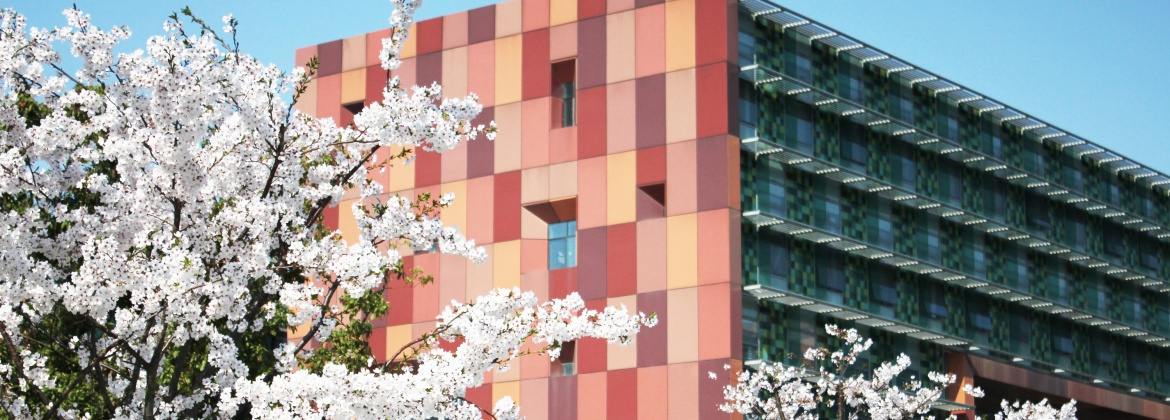
\includegraphics[height=\paperheight,width=\paperwidth,keepaspectratio=FALSE]{bgxp.jpg}};} % bdbg-1.jpeg

\titlegraphic{
\includegraphics[width=1.7cm]{xjtluicon.jpg}} %stat-right.png
\ifLuaTeX
  \usepackage{selnolig}  % disable illegal ligatures
\fi

\begin{document}
\frame{\titlepage}

\begin{frame}[fragile]{选项说明:\texttt{slide\_level:\ 3}}
\protect\hypertarget{ux9009ux9879ux8bf4ux660eslide_level-3}{}
\begin{verbatim}
1. Section title 
# 节标题

2. Subsection title
## 子节标题

3. Frame title
### 幻灯片标题

4. Block title 
#### 块标题
\end{verbatim}
\end{frame}

\begin{frame}{报告提纲}
\protect\hypertarget{ux62a5ux544aux63d0ux7eb2}{}
\tableofcontents
\end{frame}

\hypertarget{ux5b66ux672fux5e7bux706fux7247ux5236ux4f5c}{%
\section{学术幻灯片制作}\label{ux5b66ux672fux5e7bux706fux7247ux5236ux4f5c}}

\hypertarget{ux76f8ux5173ux4ecbux7ecd}{%
\subsection{相关介绍}\label{ux76f8ux5173ux4ecbux7ecd}}

\begin{frame}[fragile]{强大的Markdown+R+Beamer}
\protect\hypertarget{ux5f3aux5927ux7684markdownrbeamer}{}
\begin{itemize}
\item
  Beamer

\begin{verbatim}
Beamer是 LaTeX 上用来制作演示文档的一个套件。
\end{verbatim}
\item
  markdown

\begin{verbatim}
Markdown是一种轻量级的标记性语言。
\end{verbatim}
\item
  knitr + pandoc

\begin{verbatim}
实现文档转换, knitr支持多种语言引擎,包括R, Python
\end{verbatim}
\end{itemize}

\begin{block}{knitr + pandoc}
\protect\hypertarget{knitr-pandoc}{}
R Markdown + Beamer
\(\underset{\text{pandoc}}{\overset{\text{knitr}}{\Longrightarrow}}\)
Perfect Academic Presentation!
\end{block}
\end{frame}

\begin{frame}{原理}
\protect\hypertarget{ux539fux7406}{}
\begin{itemize}
\tightlist
\item
  knitr+ pandoc
\end{itemize}

\begin{figure}[h]

{\centering 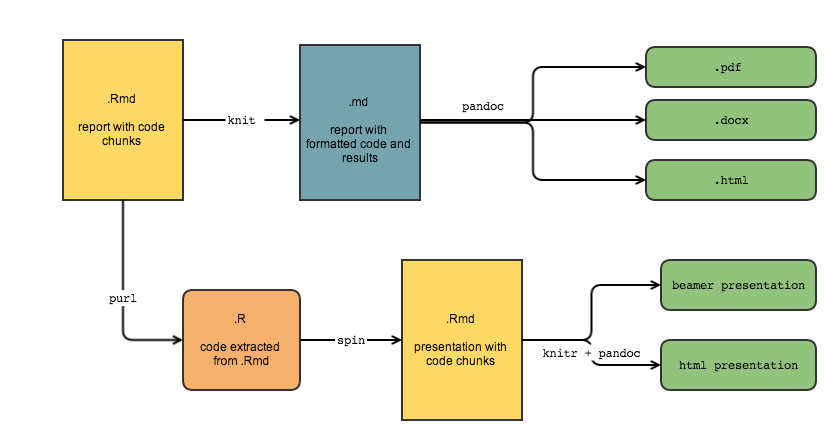
\includegraphics[width=0.65\linewidth]{./figures/knitr-workflow} 

}

\caption{Knitr workflow}\label{fig:unnamed-chunk-2}
\end{figure}
\end{frame}

\begin{frame}{基本要求}
\protect\hypertarget{ux57faux672cux8981ux6c42}{}
\begin{itemize}
\tightlist
\item
  环境安装

  \begin{itemize}
  \tightlist
  \item
    R
  \item
    knitr
  \item
    Rstudio
  \item
    \TeX{}Live (C\TeX{}套装, mactex)
  \end{itemize}
\item
  预备知识:

  \begin{itemize}
  \tightlist
  \item
    Mardown/Rmarkdown基础
  \item
    \LaTeX{}基础
  \item
    Beamer基础
  \item
    R基础
  \end{itemize}
\end{itemize}
\end{frame}

\begin{frame}[fragile]{一张幻灯片的式样}
\protect\hypertarget{ux4e00ux5f20ux5e7bux706fux7247ux7684ux5f0fux6837}{}
\begin{verbatim}
# 一级标题为对应TeX的section

## 二级标题为对应TeX的subsection

### 三级标题为Beamer幻灯片的标题,对应TeX的\frametitle{}

#### 四级标题为Beamer中块(block)标题

*Hello, R Markdown!*
\end{verbatim}
\end{frame}

\begin{frame}[fragile]{等价于Beamer中代码}
\protect\hypertarget{ux7b49ux4ef7ux4e8ebeamerux4e2dux4ee3ux7801}{}
\begin{verbatim}
\section{一级标题section}
\subsection{二级标题subsection}
\frame{
\frametitle{幻灯片的标题}
\begin{block}{Block标题}
\textit{Hello, R Markdown!}
\end{Block}
}
\end{verbatim}
\end{frame}

\begin{frame}{正文中下面的命令(环境)就不能/不必用了}
\protect\hypertarget{ux6b63ux6587ux4e2dux4e0bux9762ux7684ux547dux4ee4ux73afux5883ux5c31ux4e0dux80fdux4e0dux5fc5ux7528ux4e86}{}
\begin{itemize}
\tightlist
\item
  section
\item
  subsection
\item
  frame
\item
  列表类环境:

  \begin{itemize}
  \tightlist
  \item
    enumerate
  \item
    itemize
  \item
    list
  \item
    description
  \end{itemize}
\end{itemize}
\end{frame}

\hypertarget{beamerux5e7bux706fux7247ux7684ux4e3bux8981ux6784ux6210}{%
\section{Beamer幻灯片的主要构成}\label{beamerux5e7bux706fux7247ux7684ux4e3bux8981ux6784ux6210}}

\hypertarget{ux5e38ux7528ux8981ux7d20ux8bbeux5b9a}{%
\subsection{常用要素设定}\label{ux5e38ux7528ux8981ux7d20ux8bbeux5b9a}}

\begin{frame}[fragile]{字体与颜色设定}
\protect\hypertarget{ux5b57ux4f53ux4e0eux989cux8272ux8bbeux5b9a}{}
\begin{itemize}
\tightlist
\item
  用Markdown设定
\end{itemize}

\begin{verbatim}
    **这是粗体**
\end{verbatim}

\textbf{这是粗体},\emph{这是斜体}

\begin{itemize}
\tightlist
\item
  用\TeX{}的命令
\end{itemize}

\begin{verbatim}
  \textbf{这是黑体},\textcolor{red}{\bf 这是红色黑体}
\end{verbatim}

\textbf{这是黑体},\textcolor{red}{\bf 这是红色黑体}
\end{frame}

\begin{frame}[fragile]{有序列表设定}
\protect\hypertarget{ux6709ux5e8fux5217ux8868ux8bbeux5b9a}{}
\begin{block}{有序列表(代码)}
\protect\hypertarget{ux6709ux5e8fux5217ux8868ux4ee3ux7801}{}
\begin{verbatim}
1.  one
2.  two
3.  three
\end{verbatim}
\end{block}

\begin{block}{有序列表(结果)}
\protect\hypertarget{ux6709ux5e8fux5217ux8868ux7ed3ux679c}{}
\begin{enumerate}
\tightlist
\item
  one
\item
  two
\item
  three
\end{enumerate}
\end{block}
\end{frame}

\begin{frame}[fragile]{无序列表设定}
\protect\hypertarget{ux65e0ux5e8fux5217ux8868ux8bbeux5b9a}{}
\begin{block}{无序列表(代码)}
\protect\hypertarget{ux65e0ux5e8fux5217ux8868ux4ee3ux7801}{}
\begin{verbatim}
* fruits
    + apples
        - macintosh
        - red delicious
    + pears
\end{verbatim}
\end{block}

\begin{block}{无序列表(结果)}
\protect\hypertarget{ux65e0ux5e8fux5217ux8868ux7ed3ux679c}{}
\begin{itemize}
\tightlist
\item
  fruits

  \begin{itemize}
  \tightlist
  \item
    apples

    \begin{itemize}
    \tightlist
    \item
      macintosh
    \item
      red delicious
    \end{itemize}
  \item
    pears
  \end{itemize}
\end{itemize}
\end{block}
\end{frame}

\hypertarget{rux4ee3ux7801ux4e0eux5206ux6790ux7ed3ux679cux8f93ux51fa}{%
\subsection{R代码与分析结果输出}\label{rux4ee3ux7801ux4e0eux5206ux6790ux7ed3ux679cux8f93ux51fa}}

\begin{frame}[fragile]{统计量输出}
\protect\hypertarget{ux7edfux8ba1ux91cfux8f93ux51fa}{}
\begin{Shaded}
\begin{Highlighting}[]
\FunctionTok{summary}\NormalTok{(cars)}
\end{Highlighting}
\end{Shaded}

\begin{verbatim}
     speed           dist       
 Min.   : 4.0   Min.   :  2.00  
 1st Qu.:12.0   1st Qu.: 26.00  
 Median :15.0   Median : 36.00  
 Mean   :15.4   Mean   : 42.98  
 3rd Qu.:19.0   3rd Qu.: 56.00  
 Max.   :25.0   Max.   :120.00  
\end{verbatim}
\end{frame}

\begin{frame}[fragile]{图形输出}
\protect\hypertarget{ux56feux5f62ux8f93ux51fa}{}
\begin{Shaded}
\begin{Highlighting}[]
\FunctionTok{plot}\NormalTok{(pressure)}
\end{Highlighting}
\end{Shaded}

\begin{figure}[h]

{\centering 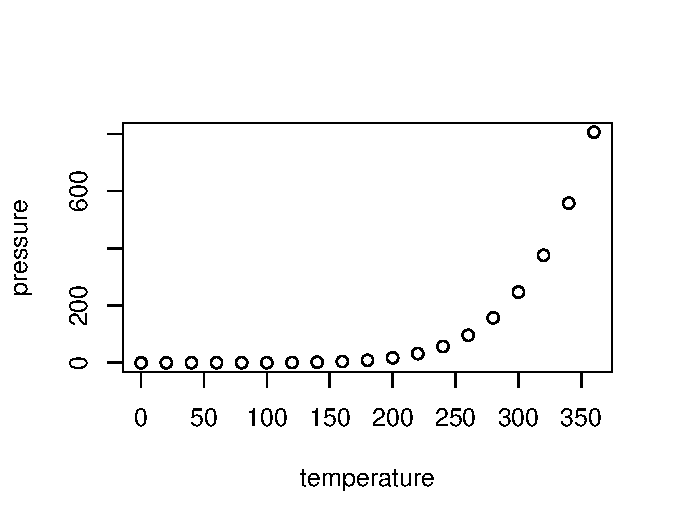
\includegraphics[width=0.55\linewidth]{figures/pressure-1} 

}

\caption{Pressure}\label{fig:pressure}
\end{figure}
\end{frame}

\begin{frame}[fragile]{表格输出: 使用kable}
\protect\hypertarget{ux8868ux683cux8f93ux51fa-ux4f7fux7528kable}{}
\begin{block}{R代码}
\protect\hypertarget{rux4ee3ux7801}{}
\begin{Shaded}
\begin{Highlighting}[]
\NormalTok{n }\OtherTok{\textless{}{-}} \DecValTok{100}\NormalTok{; x }\OtherTok{\textless{}{-}} \FunctionTok{rnorm}\NormalTok{(n)}
\NormalTok{y }\OtherTok{\textless{}{-}} \DecValTok{2}\SpecialCharTok{*}\NormalTok{x }\SpecialCharTok{+} \FunctionTok{rnorm}\NormalTok{(n)}
\NormalTok{out }\OtherTok{\textless{}{-}} \FunctionTok{lm}\NormalTok{(y }\SpecialCharTok{\textasciitilde{}}\NormalTok{ x)}
\FunctionTok{library}\NormalTok{(knitr)}
\FunctionTok{kable}\NormalTok{(}\AttributeTok{caption =} \StringTok{"kable"}\NormalTok{, }\FunctionTok{summary}\NormalTok{(out)}\SpecialCharTok{$}\NormalTok{coef, }\AttributeTok{digits=}\DecValTok{2}\NormalTok{)}
\end{Highlighting}
\end{Shaded}

\begin{longtable}[]{@{}lrrrr@{}}
\caption{kable}\tabularnewline
\toprule
& Estimate & Std. Error & t value &
Pr(\textgreater\textbar t\textbar) \\
\midrule
\endfirsthead
\toprule
& Estimate & Std. Error & t value &
Pr(\textgreater\textbar t\textbar) \\
\midrule
\endhead
(Intercept) & -0.02 & 0.1 & -0.22 & 0.82 \\
x & 1.96 & 0.1 & 20.19 & 0.00 \\
\bottomrule
\end{longtable}
\end{block}
\end{frame}

\begin{frame}[fragile]{表格输出: 使用xtable}
\protect\hypertarget{ux8868ux683cux8f93ux51fa-ux4f7fux7528xtable}{}
\begin{block}{R代码}
\protect\hypertarget{rux4ee3ux7801-1}{}
\begin{Shaded}
\begin{Highlighting}[]
\NormalTok{n }\OtherTok{\textless{}{-}} \DecValTok{100}
\NormalTok{x }\OtherTok{\textless{}{-}} \FunctionTok{rnorm}\NormalTok{(n)}
\NormalTok{y }\OtherTok{\textless{}{-}} \DecValTok{2}\SpecialCharTok{*}\NormalTok{x }\SpecialCharTok{+} \FunctionTok{rnorm}\NormalTok{(n)}
\NormalTok{out }\OtherTok{\textless{}{-}} \FunctionTok{lm}\NormalTok{(y }\SpecialCharTok{\textasciitilde{}}\NormalTok{ x)}
\FunctionTok{library}\NormalTok{(xtable)}
\NormalTok{lmcoef}\OtherTok{\textless{}{-}} \FunctionTok{xtable}\NormalTok{(}\FunctionTok{summary}\NormalTok{(out)}\SpecialCharTok{$}\NormalTok{coef, }
                \AttributeTok{digits=}\FunctionTok{c}\NormalTok{(}\DecValTok{0}\NormalTok{, }\DecValTok{2}\NormalTok{, }\DecValTok{2}\NormalTok{, }\DecValTok{1}\NormalTok{, }\DecValTok{2}\NormalTok{))}
\FunctionTok{print}\NormalTok{(lmcoef)}
\end{Highlighting}
\end{Shaded}
\end{block}
\end{frame}

\begin{frame}[fragile]{表格输出: 使用xtable}
\protect\hypertarget{ux8868ux683cux8f93ux51fa-ux4f7fux7528xtable-1}{}
\begin{block}{自动转化为\TeX{}代码}
\protect\hypertarget{ux81eaux52a8ux8f6cux5316ux4e3aux4ee3ux7801}{}
\small

\begin{verbatim}
\begin{table}[ht]
\centering
\begin{tabular}{rrrrr}
  \hline
 & Estimate & Std. Error & t value & Pr($>$$|$t$|$) \\ 
  \hline
(Intercept) & -0.03 & 0.09 & -0.3 & 0.73 \\ 
  x & 1.92 & 0.08 & 23.0 & 0.00 \\ 
   \hline
\end{tabular}
\caption{xtable} 
\end{table}
\end{verbatim}
\end{block}
\end{frame}

\begin{frame}[fragile]{输出表格}
\protect\hypertarget{ux8f93ux51faux8868ux683c}{}
\begin{block}{例(续)}
\protect\hypertarget{ux4f8bux7eed}{}
\small

\begin{Shaded}
\begin{Highlighting}[]
\FunctionTok{print}\NormalTok{(lmcoef,}\AttributeTok{caption.placement=}\StringTok{"top"}\NormalTok{,}\AttributeTok{comment=}\ConstantTok{FALSE}\NormalTok{)}
\end{Highlighting}
\end{Shaded}

\begin{table}[ht]
\centering
\caption{xtable} 
\begin{tabular}{rrrrr}
  \hline
 & Estimate & Std. Error & t value & Pr($>$$|$t$|$) \\ 
  \hline
(Intercept) & -0.03 & 0.09 & -0.3 & 0.73 \\ 
  x & 1.92 & 0.08 & 23.0 & 0.00 \\ 
   \hline
\end{tabular}
\end{table}
\end{block}
\end{frame}

\begin{frame}[fragile]{数学公式}
\protect\hypertarget{ux6570ux5b66ux516cux5f0f}{}
\begin{itemize}
\item
  行内公式 \texttt{\$x\^{}2+y\^{}2=1\$} 或
  \texttt{\textbackslash{}(x\^{}2+y\^{}2=1\textbackslash{})}:
  \(x^2+y^2=1\).
\item
  独立行公式:
\end{itemize}

\begin{verbatim}
$$
\oint_C x^3\, dx + 4y^2\, dy
$$
\end{verbatim}

\[
\oint_C x^3\, dx + 4y^2\, dy
\]
\end{frame}

\begin{frame}[fragile]{双栏排版}
\protect\hypertarget{ux53ccux680fux6392ux7248}{}
\begin{columns}[T]
\begin{column}{0.35\textwidth}
\begin{Shaded}
\begin{Highlighting}[]
\NormalTok{  n }\OtherTok{\textless{}{-}} \DecValTok{100}\NormalTok{; x }\OtherTok{\textless{}{-}} \FunctionTok{rnorm}\NormalTok{(n)}
\NormalTok{  y }\OtherTok{\textless{}{-}} \DecValTok{2}\SpecialCharTok{*}\NormalTok{x }\SpecialCharTok{+} \FunctionTok{rnorm}\NormalTok{(n)}
\NormalTok{  out }\OtherTok{\textless{}{-}} \FunctionTok{lm}\NormalTok{(y }\SpecialCharTok{\textasciitilde{}}\NormalTok{ x)}
  \FunctionTok{library}\NormalTok{(knitr)}
  \FunctionTok{kable}\NormalTok{(}\AttributeTok{caption =} \StringTok{"kable"}\NormalTok{, }
        \FunctionTok{summary}\NormalTok{(out)}\SpecialCharTok{$}\NormalTok{coef, }
        \AttributeTok{digits=}\DecValTok{2}\NormalTok{)}
\end{Highlighting}
\end{Shaded}
\end{column}

\begin{column}{0.05\textwidth}
~
\end{column}

\begin{column}{0.65\textwidth}
\begin{longtable}[]{@{}lrrrr@{}}
\caption{kable}\tabularnewline
\toprule
& Estimate & Std. Error & t value &
Pr(\textgreater\textbar t\textbar) \\
\midrule
\endfirsthead
\toprule
& Estimate & Std. Error & t value &
Pr(\textgreater\textbar t\textbar) \\
\midrule
\endhead
(Intercept) & 0.13 & 0.09 & 1.43 & 0.16 \\
x & 1.98 & 0.08 & 26.32 & 0.00 \\
\bottomrule
\end{longtable}
\end{column}
\end{columns}

\begin{itemize}
\item
  对于纯文字及图表还使用\TeX{}的

  \begin{itemize}
  \item
    minipage环境
  \item
    columns环境
  \end{itemize}
\end{itemize}
\end{frame}

\begin{frame}[c]{}
% \emph {\Huge{\color{blue}\centerline{\CJKfontspec[FakeSlant = 0.2]{STSong}谢谢!} }  }
 \Huge{\color{blue}\centerline{谢谢!} }  
 \emph {\Huge{\color{blue}\centerline{Thank you!} }  }
\end{frame}

\end{document}
